\section{Descrizione Design Pattern }
I \glossaryItem{Design Pattern} sono un modello logico da applicare per la soluzione di problemi
ricorrenti. L’impiego di questi modelli rende l'architettura più manutenibile. Verranno
di seguito illustrati i Design Pattern implementati nella costruzione dell’architettura di
alto livello, divisi per categoria di applicazione:
	\subsection{Design Pattern Architetturali}
	
		\subsubsection{MVVM}
		\begin{figure}[H]
		\centering
		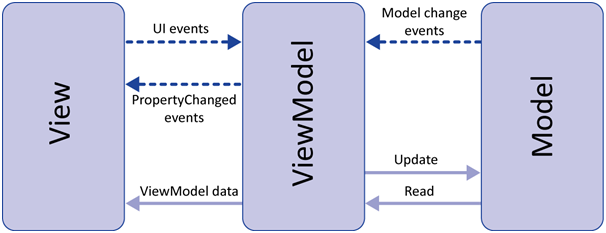
\includegraphics[width=0.5\linewidth]{GraficiAppendici/mvvm.png}
		\caption{Diagramma del Design Pattern MVVM}
	\end{figure}
		\begin{itemize}
		\item \textbf{Scopo}: Lo scopo del MVVM è quello di separare le seguenti componenti in modo da non mescolare il codice della logica con quella dell'interfaccia utente:
		\begin{itemize}
		\item Model - rappresenta il punto di accesso ai dati. Trattasi di una o più classi che leggono dati dal DB, oppure da un servizio Web di qualsivoglia natura;
		\item View - rappresenta la vista dell’applicazione, l’interfaccia grafica che mostrerà i dati;
		\item ViewModel - è il punto di incontro tra la View e il Model: i dati ricevuti da quest’ultimo sono elaborati per essere presentati e passati alla View.
		\end{itemize}

		\item \textbf{Motivazione}: MVVM è stato progettato per utilizzare le funzioni di binding dei dati in WPF (Windows Presentation Foundation) per facilitare la separazione della view dal resto del modello, rimuovendo praticamente tutti i codici \glossaryItem{GUI} dal livello di visualizzazione. Invece di richiedere agli sviluppatori di \glossaryItem{user experience} (UX) di scrivere il codice \glossaryItem{GUI}, possono utilizzare il linguaggio di marcatura dei framework e creare connessioni di dati al modello di visualizzazione, che viene scritto e gestito dagli sviluppatori di applicazioni. La separazione dei ruoli consente ai progettisti interattivi di concentrarsi sulle esigenze UX anziché sulla programmazione della logica aziendale. Gli strati di un'applicazione possono quindi essere sviluppati in più flussi di lavoro per una maggiore produttività. Anche quando un singolo sviluppatore lavora sull'intera base di codice, una corretta separazione della vista dal modello è più produttiva, poiché l'interfaccia utente tipicamente cambia ed è in ritardo nel ciclo di sviluppo in base ai feedback degli utenti finali. 
\item \textbf{Applicabilità}: il modello MVVM è in definitiva la moderna struttura del modello MVC, quindi l'obiettivo principale è sempre lo stesso per fornire una netta separazione tra logica di dominio e livello di presentazione. Esso è applicabile nei seguenti casi:
\begin{itemize}
\item Quando si vuole ottenere la vera separazione tra la view e la model oltre a conseguire la separazione e l'efficienza che si guadagna ad averla;
\item Quando si vuole codice manutenibile e estensibile. 
\end{itemize}
		\end{itemize}
	
		\subsubsection{Three-Tier}
		\begin{figure}[H]
		\centering
		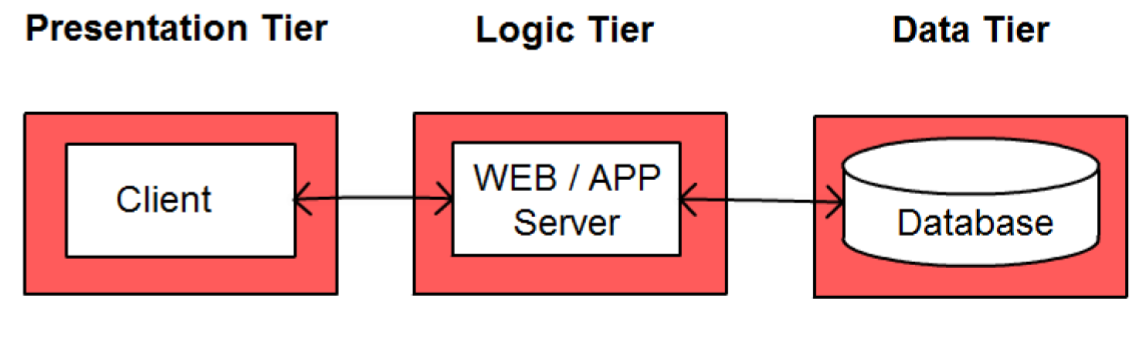
\includegraphics[width=0.6\linewidth]{GraficiAppendici/3-tier.png}
		\caption{Diagramma del Design Pattern Three-Tier}
	\end{figure}
		\begin{itemize}
		\item \textbf{Scopo}: tale design pattern permette una disgiunzione tra i vari gruppi di
entità che cooperano nell’erogazione del servizio. Esisterà un livello che si occuperà
di interagire con il cliente offrendo l’interfaccia grafica, un altro livello che gestirà
di eseguire la parte algoritmica dell’applicazione e un altro livello che si occuperà di
persistere i dati e recuperarli. Ogni livello comunicherà solo con i livelli adiacenti.

	\item \textbf{Motivazione}: si tratta di un pattern molto utilizzato nelle applicazioni web perché rende l’applicazione flessibile, riutilizzabile e scalabile. Con la separazione di un’applicazione in livelli, gli sviluppatori, per modificare o aggiungere funzionalità, possono infatti modificare solo uno specifico livello piuttosto che dover riscrivere l’intera applicazione. Ciò garantisce dunque una maggiore semplicità di progettazione/implementazione secondo la filosofia del divide et impera ed una maggiore manutenibilità.
		\end{itemize}
	\subsection{Design Pattern Creazionali}
	
		\subsubsection{Factory Method}
		\begin{figure}[H]
		\centering
		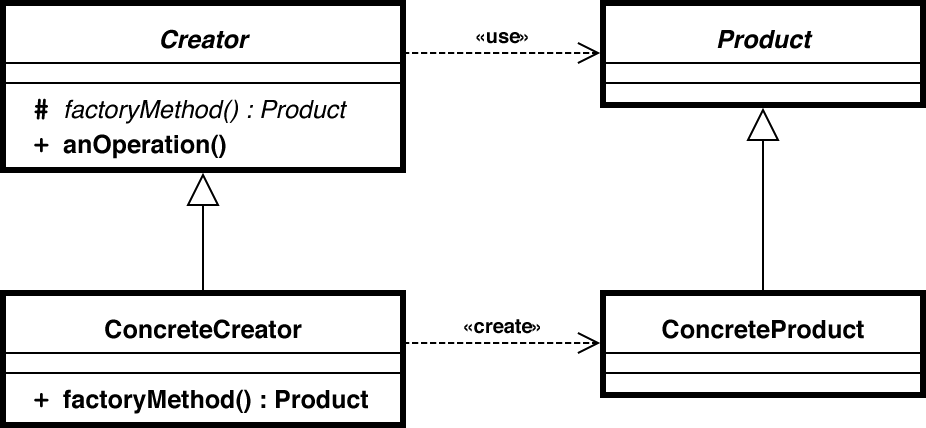
\includegraphics[width=0.5\linewidth]{GraficiAppendici/factory.png}
		\caption{Diagramma del Design Pattern Factory method}
	\end{figure}
		\begin{itemize}
		\item \textbf{Scopo}: il design pattern Factory Method indirizza il problema della creazione
di oggetti senza specificarne l’esatta classe, fornendo un’interfaccia per creare un oggetto, ma lasciando che le sottoclassi decidano quale oggetto istanziare. Definisce un’interfaccia (Creator) per ottenere una nuova istanza di un oggetto (Product). Delega ad una classe derivata (ConcreteCreator) la scelta di quale classe istanziare (ConcreteProduct).
		\item \textbf{Motivazione}: la creazione di un oggetto può, spesso, richiedere processi complessi la cui collocazione all’interno della classe di composizione potrebbe non essere appropriata. Esso può, inoltre, comportare duplicazione di codice, richiedere informazioni non accessibili alla classe di composizione, o non fornire un sufficiente livello di astrazione.
Il Factory Method indirizza questi problemi definendo un metodo separato per la creazione degli oggetti. Tale metodo può essere ridefinito dalle sottoclassi per definire il tipo derivato di prodotto che verrà effettivamente creato.
		\item \textbf{Applicabilità}: tale design pattern verrà utilizzato nei seguenti casi:
		\begin{itemize}
		\item si desidera che la creazione di un oggetto non precluda il suo riuso senza una significativa duplicazione di codice;
		\item si desidera che la creazione di un oggetto non richieda l’accesso ad informazioni o risorse che non dovrebbero essere contenute nella classe di composizione;
		\item si desidera che la gestione del ciclo di vita degli oggetti gestiti debba essere centralizzata in modo da assicurare un comportamento consistente all’interno dell’applicazione.
		\end{itemize}
		\end{itemize}				
		
	\subsection{Design Pattern Strutturali}

		\subsubsection{Decorator}
		\begin{figure}[H]
		\centering
		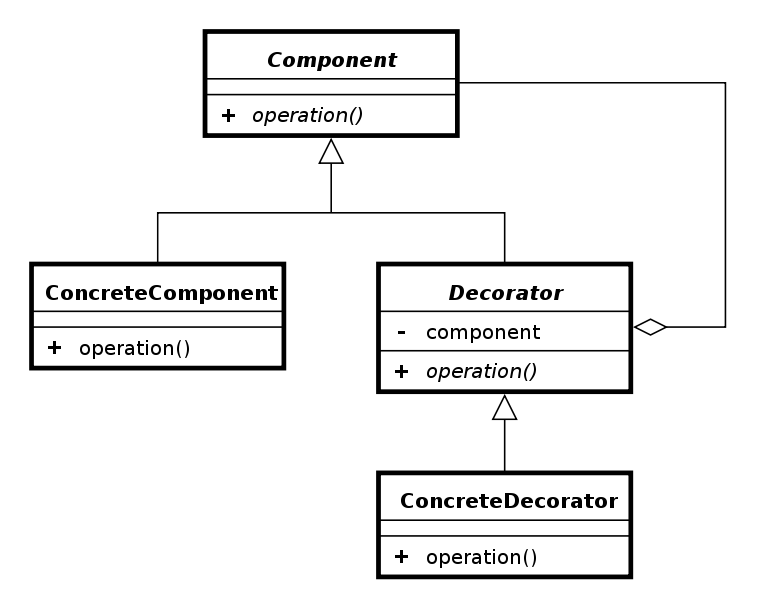
\includegraphics[width=0.5\linewidth]{GraficiAppendici/decorator.png}
		\caption{Diagramma del Design Pattern Decorator}
	\end{figure}
	\begin{itemize}
	\item \textbf{Scopo}: aggiungere dinamicamente responsabilità a un oggetto. I Decorator forniscono
un’alternativa flessibile alla definizione di sottoclassi come strumento per l’estensione delle funzionalità;
	\item \textbf{Motivazione}: talvolta si vogliono aggiungere responsabilità a singoli oggetti e
non a un’intera classe. Un modo per aggiungere responsabilità consiste nel racchiudere il componente da
decorare in un altro. L’oggetto contenitore è chiamato Decorator. Il Decorator ha un interfaccia conforme a quella dell’elemento decorato, in modo da rendere trasparente la sua presenza ai client. Il decorator trasferisce le richieste al componente decorato e può svolgere azioni aggiuntive prima o dopo il trasferimento della richiesta;
	\item \textbf{Applicabilità}: il pattern Decorator può essere utilizzato nei seguenti casi:
	\begin{itemize}
	\item Si vuole poter aggiungere responsabilità a singoli oggetti dinamicamente ed in modo trasparente;
	\item Si vuole poter togliere responsabilità agli oggetti;
	\item Si vuole definire un gran numero di estensioni indipendenti.
	\end{itemize}
\end{itemize}			
		
		\subsubsection{Facade}
		\begin{figure}[H]
		\centering
		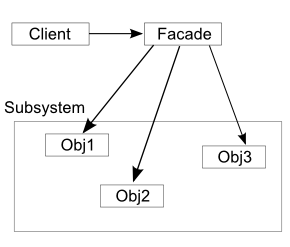
\includegraphics[width=0.4\linewidth]{GraficiAppendici/facade.png}
		\caption{Diagramma del Design Pattern Facade}
	\end{figure}
		\begin{itemize}
		\item \textbf{Scopo}: fornire un’interfaccia unificata per un insieme di interfacce presenti in un
sottosistema. Definisce un’interfaccia di livello più alto che rende il sottosistema più semplice da utilizzare;
		\item \textbf{Motivazione}: suddividere un sistema in sottosistemi aiuta a ridurne la complessità.
Un obiettivo comune di progettazione è la minimizzazione delle comunicazioni e delle dipendenza fra i diversi sottosistemi. Un modo per raggiungere questo obiettivo è introdurre un oggetto facade, che fornisce un’interfaccia unica e semplificata per accedere alle funzionalità offerte da un sottosistema;
		\item \textbf{Applicabilità}: il pattern Facade può essere utilizzato nei seguenti casi:
		\begin{itemize}
		\item Quando si vuole fornire un’interfaccia semplice a un sottosistema complesso poiché fornisce una vista semplice di base su un sottosistema che si rivela essere sufficiente per la maggior parte dei client;
		\item Nei casi in cui ci sono molte dipendenze fra i client e le classi che implementano un’astrazione in quanto si disaccoppia il sottosistema dai client e dagli altri sistemi, promuovendo portabilità e indipendenza dei sottosistemi;
		\item Quando si vogliono organizzare i sottosistemi in una struttura a livelli.
		\end{itemize}

		\end{itemize}
	
	\subsection{Design Pattern Comportamentali}
	
		\subsubsection{Dependency Injection}
		\begin{figure}[H]
		\centering
		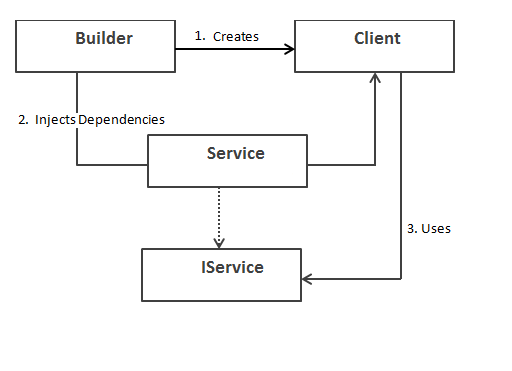
\includegraphics[width=0.5\linewidth]{GraficiAppendici/dependency.png}
		\caption{Diagramma del Design Pattern Dependency Injection}
	\end{figure}
		\begin{itemize}
		\item \textbf{Scopo}: Il Dependency Injection è un Design Pattern che permette la separazione del comportamento degli oggetti dalla loro dipendenze. Invece di istanziare le classi in modo diretto ogni componente riceve i riferimenti agli altri componenti necessari come parametri nel costruttore. Un utilizzo comune è quello con i plugin che vengono caricati dinamicamente. Gli elementi coinvolti sono:
\begin{itemize}
\item Un dipendente consumatore;
\item Una dichiarazione delle dipendenze tra la componenti, definita come contratto di un interfaccia;
\item Un injector che crea istanze di classi che implementano una data dipendenza su richiesta.
\end{itemize}
Il dependent object dichiara da quali componenti dipende. L’injector decide quali classi soddisfano suoi requisiti e in caso affermativo gliele fornisce. Questa operazione può avvenire anche a runtime. Questo è un chiaro vantaggio poiché possono essere create dinamicamente diverse implementazioni di un componente software da passare allo stesso test. In questo modo il test può testare componenti diverse senza sapere che le loro implementazioni sono diverse.
\item \textbf{Motivazione}: lo scopo principale di questo pattern è quello di permettere una selezione a runtime su più implementazioni di una interfaccia dipendente. È particolarmente utile per fornire delle implementazioni di stub per componenti complesse, ma anche per gestire i plugin e per inizializzare servizi software. I test di unità comportano delle problematiche, poiché spesso richiedono la presenza di una parte di infrastruttura non ancora implementata. Il Dependency Injection semplifica il processo di testing per un istanza isolata. Poiché le componenti dichiarano le proprie dipendenze, un test può automaticamente istanziare le componenti necessarie.
\item \textbf{Applicabilità}: Di seguito vengono elencati tre modi con cui un oggetto può ricevere un riferimento da un modulo esterno:
\begin{itemize}
\item Interface injection: l’oggetto fornisce un interfaccia che gli utenti possono implementare
in modo da ottenere a runtime le dipendenze;
\item Setter injection: il dependent module espone un metodo setter che il frameworkG usa per
iniettarvi le dipendenze;
\item Constructor injection: le dipendenze vengono fornite tramite il costruttore della classe.
\end{itemize}

		\end{itemize}
		\subsubsection{Command}	
		\begin{figure}[H]
		\centering
		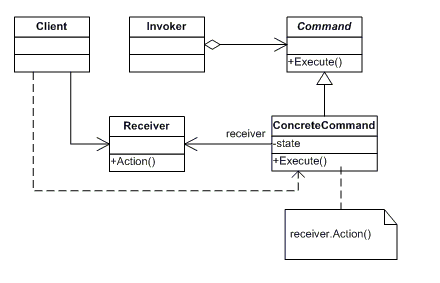
\includegraphics[width=0.6\linewidth]{GraficiAppendici/command.png}
		\caption{Diagramma del Design Pattern Command}
	\end{figure}
		\begin{itemize}
		\item \textbf{Scopo}: Incapsula una richiesta in un oggetto, consentendo di parametrizzare i
client con richieste diverse, accodare o mantenere uno storico delle richieste e gestire richieste cancellabili;
		\item \textbf{Motivazione}: Talvolta è necessario inoltrare richieste a oggetti senza conoscere
nulla dell’operazione richiesta o del destinatario della richiesta. Il pattern Command permette agli oggetti dell’ambiente di inoltrare richieste a oggetti sconosciuti dell’applicazione trasformando la richiesta in un oggetto;
		\item \textbf{Applicabilità}: Il pattern Command può essere utilizzato nei seguenti casi:
		\begin{itemize}
		\item Per parametrizzare gli oggetti rispetto a un’azione da compiere;
		\item Per specificare, accordare ed eseguire le richieste in tempi diversi;
		\item Per consentire l’annullamento di operazioni;
		\item Per organizzare un sistema in operazioni d’alto livello a loro volta basate su operazioni primitive.
		\end{itemize}

		\end{itemize}
		
	